\documentclass{beamer}
\usetheme{Frankfurt}
\setbeamertemplate{footline}[frame number]
\setbeamercovered{transparent}
\usepackage{graphicx}
\usepackage{animate}
\graphicspath{{../images/}{../videos/}{../videos/test/}}
\usepackage{tikz}



\title{SPH simulations for space defense}
\author{Maximilian Rutz}

\begin{document}
\begin{frame}[plain]
    \maketitle
\end{frame}
\begin{frame}[plain]{Roadmap}
\tableofcontents
\end{frame}
\section{Dart and Hera Missions}
\begin{frame}
	\begin{tikzpicture}[remember picture,overlay]
	\node[at=(current page.center)] {
		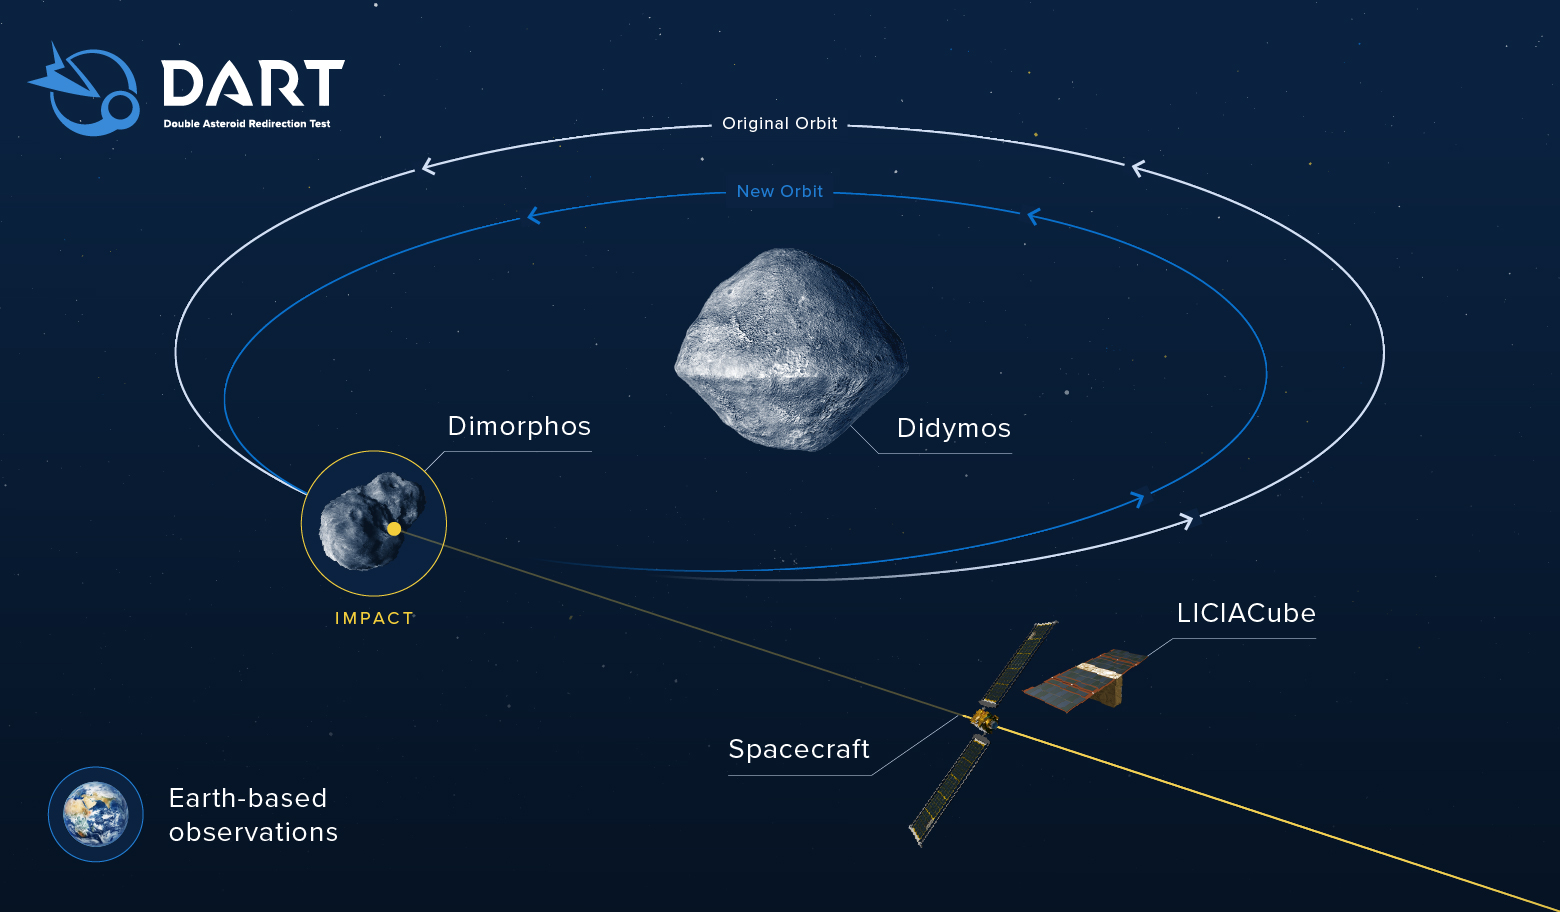
\includegraphics[keepaspectratio,
		width=\paperwidth,
		height=\paperheight]{dart_mission.jpg}};
	\end{tikzpicture}
\end{frame}
\begin{frame}{Dart Mission}
	%https://dart.jhuapl.edu/Gallery/media/graphics/lg/DART-infographic_v4.jpg
	\begin{itemize}
		\item Launch in July 2021 on a SpaceX Falcon 9 \pause
		\item Impact in fall 2022 \pause
		\item Impact at ~0.07 au to Earth, ~29 Earth-Moon, ~1/5 Earth-Mars \pause
		\item Observations with LICIACube and earth based telescopes
	\end{itemize}
\end{frame}
\begin{frame}{Hera Mission}
	\begin{tikzpicture}[remember picture,overlay]
	\node[at=(current page.center)] {
		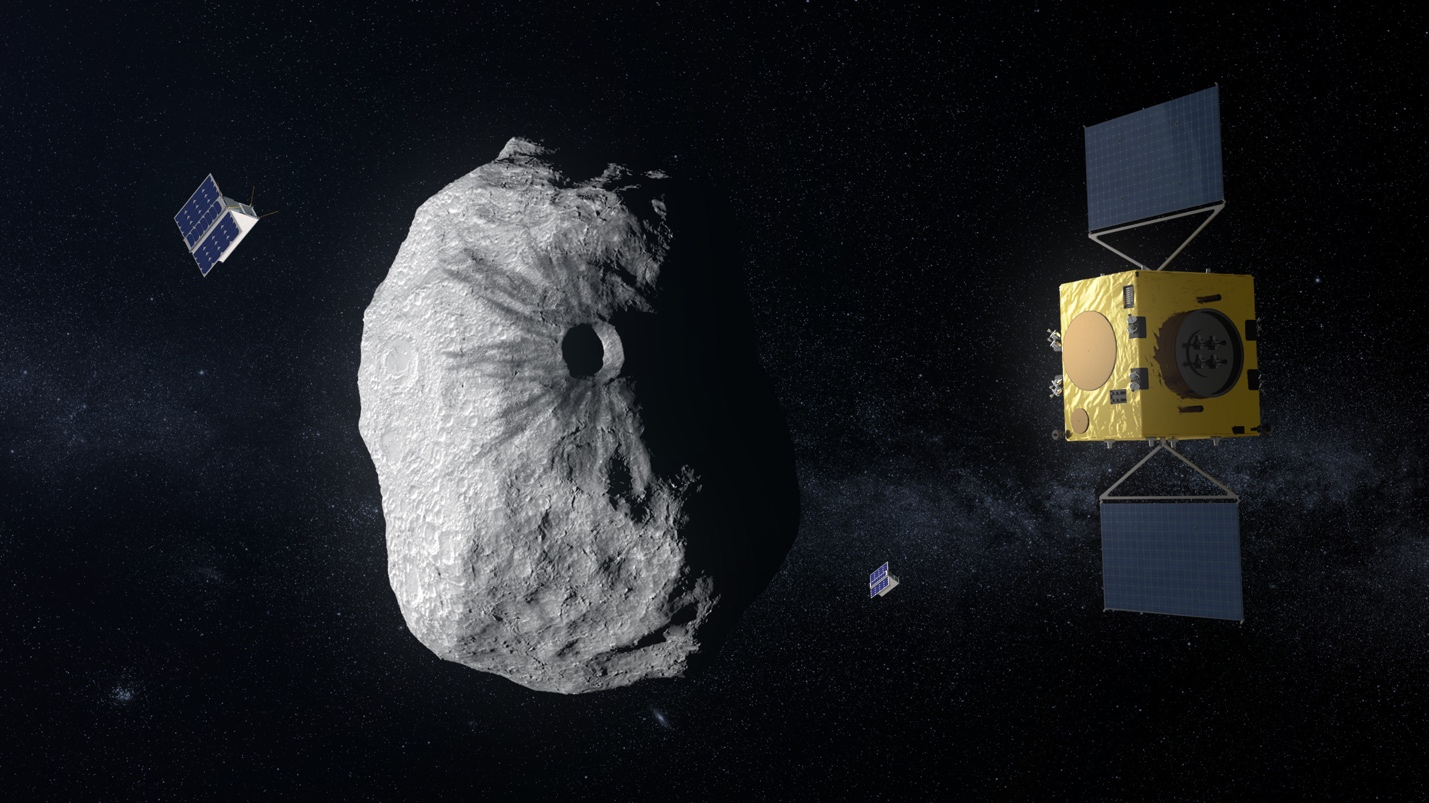
\includegraphics[keepaspectratio,
		width=\paperwidth,
		height=\paperheight]{hera_mission.jpg}};
	\end{tikzpicture}
\end{frame}
\begin{frame}{Hera Mission}
%https://www.esa.int/var/esa/storage/images/esa_multimedia/images/2018/06/testing_deflection/1%5359917-7-eng-GB/Testing_deflection_pillars.jpg
	\begin{itemize}
		\item Launch in 2024 \pause
		\item Arrival in 2026 \pause
		\item Why a second mission? \pause
		\begin{itemize}
			\item Dust cloud after impact \pause
			\item Reduce uncertainty of orbital shift \pause
			\item Politics ... \pause
		\end{itemize}
	\end{itemize}	
\end{frame}
\begin{frame}
	\begin{tikzpicture}[remember picture,overlay]
		\node[at=(current page.center)] {
		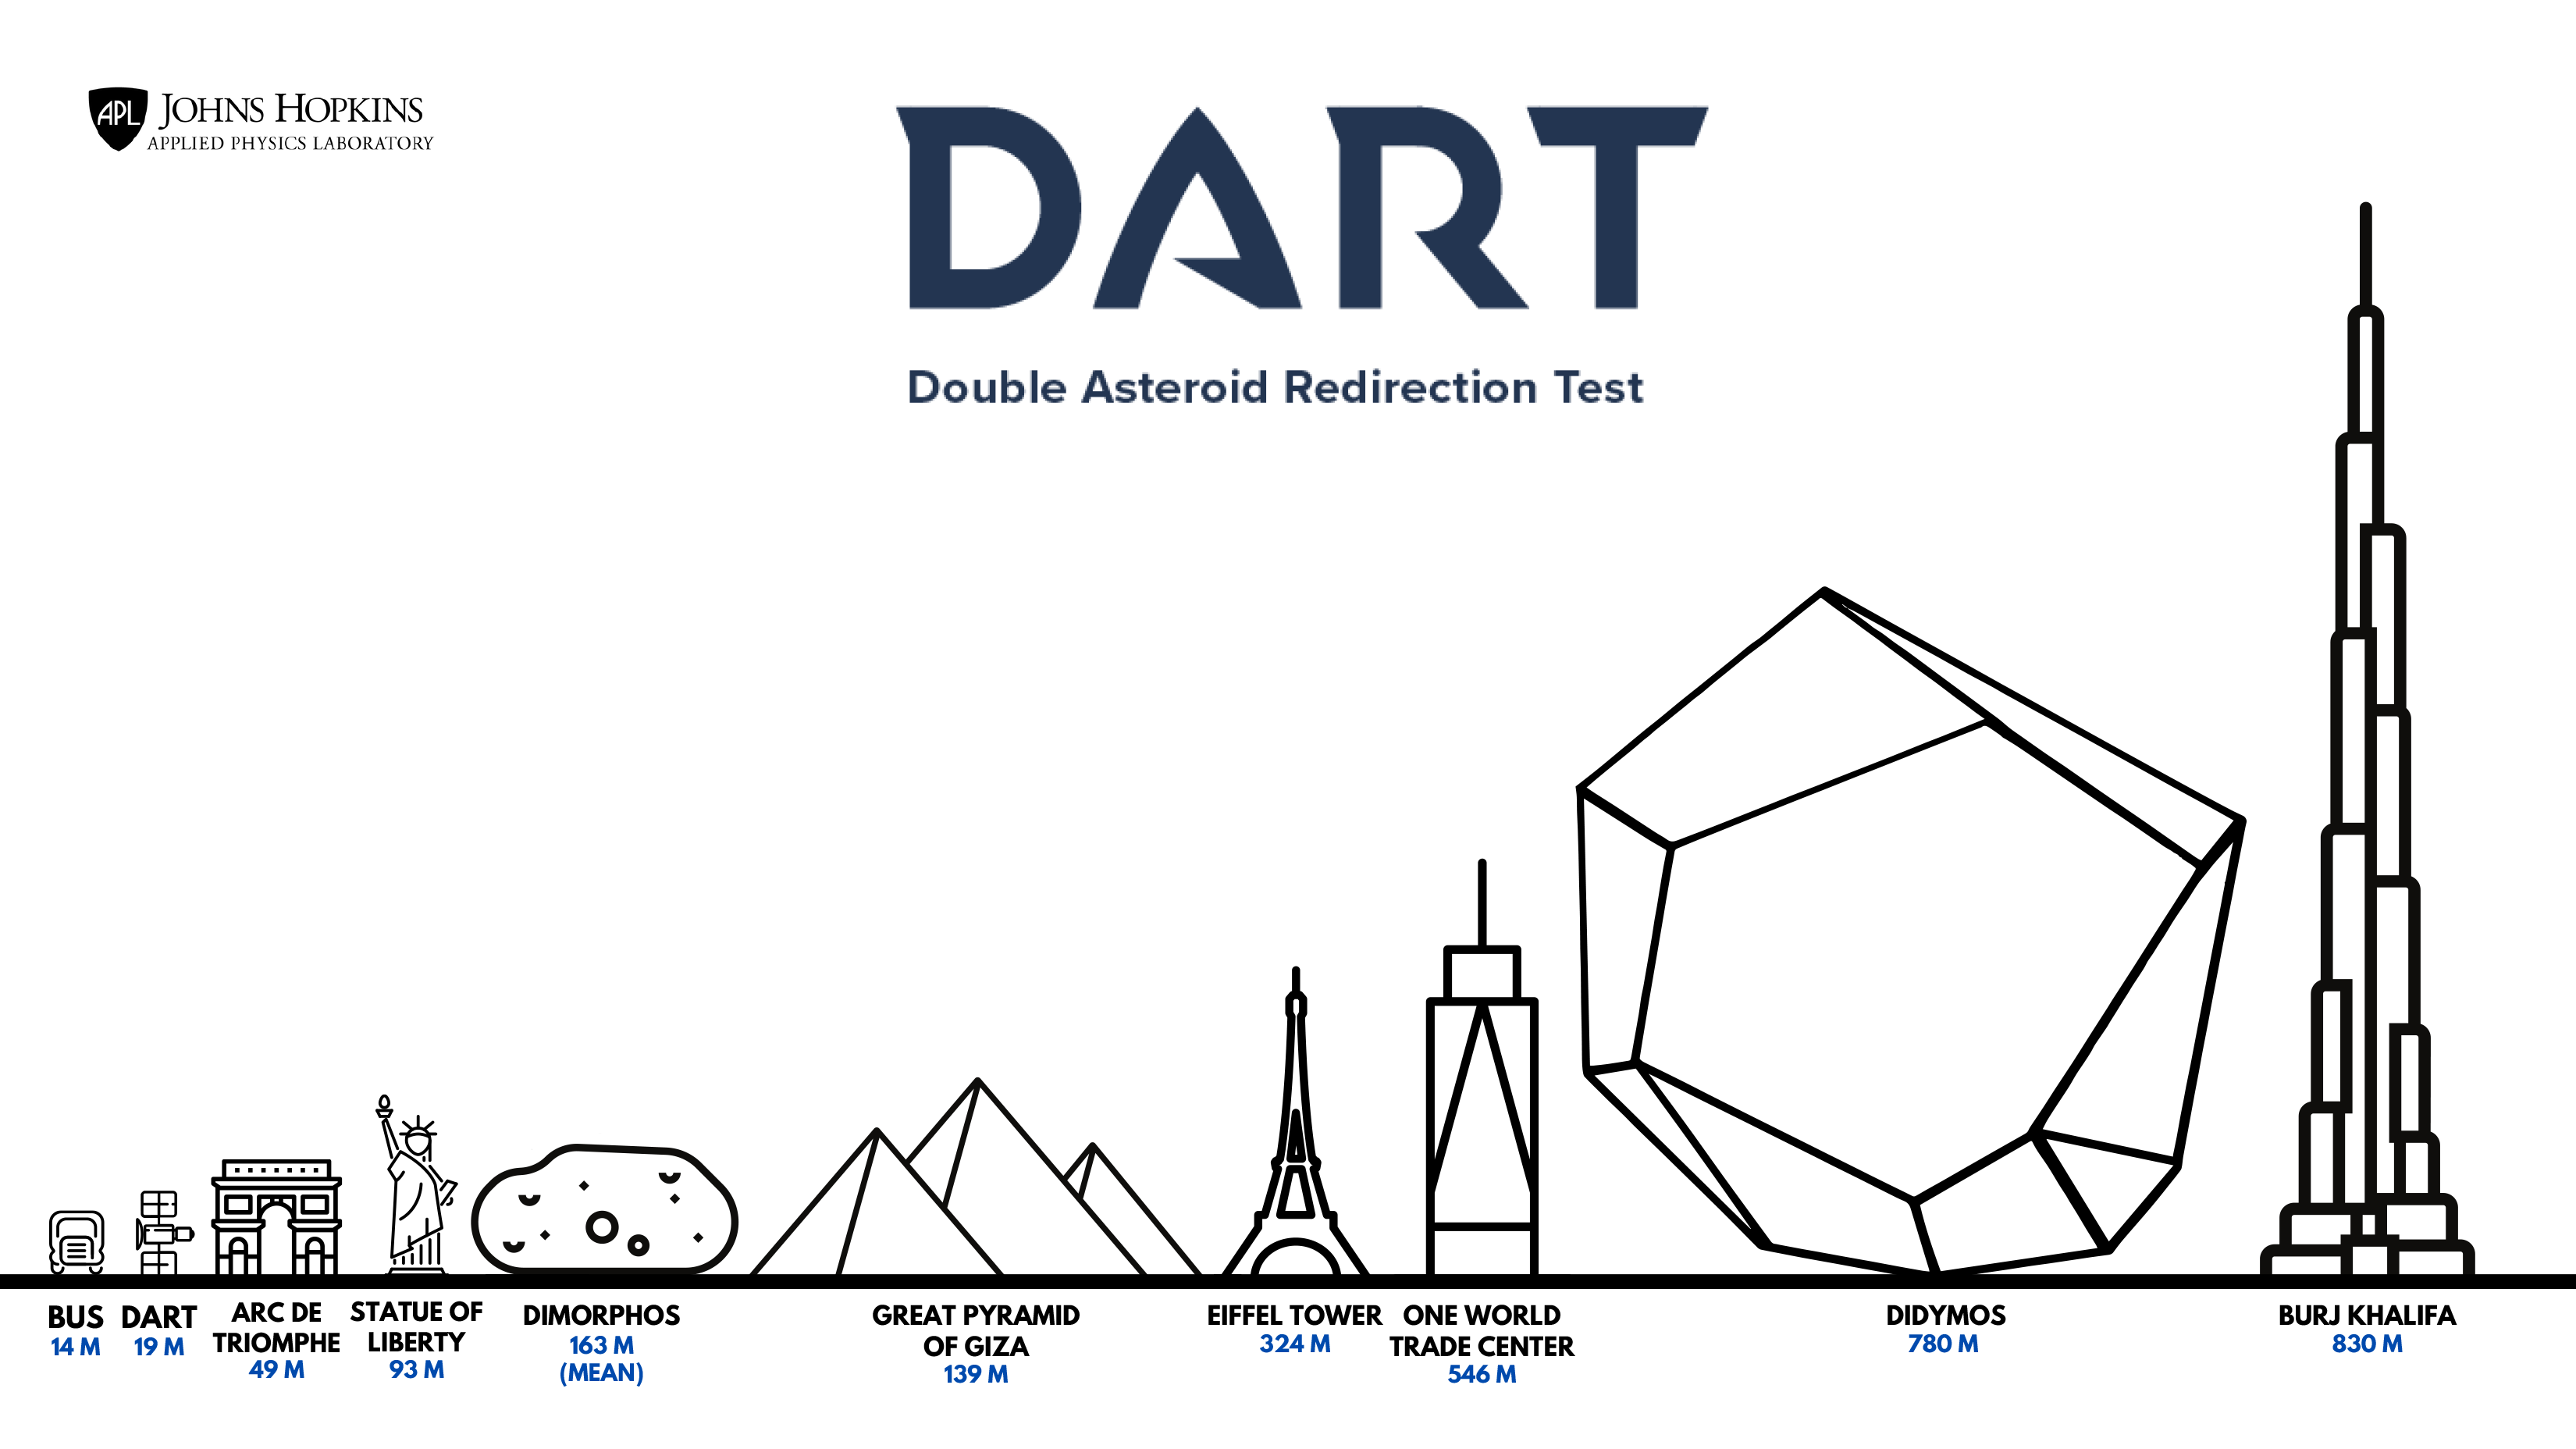
\includegraphics[keepaspectratio,
		width=\paperwidth,
		height=\paperheight]{asteroids_size.png}};
	\end{tikzpicture}
\end{frame}
\begin{frame}{Target}
	https://www.nasa.gov/planetarydefense/dart
	
	Dimorphos orbiting Didymos 
	https://dart.jhuapl.edu/Gallery/media/graphics/lg/DART%20Coloring%20Page.png
\end{frame}
\begin{frame}{Impactor}
	https://dart.jhuapl.edu/Mission/Impactor-Spacecraft.php
	\begin{itemize}
	\item 1.2 × 1.3 × 1.3 meters \pause
	\item artifical viscosity \pause

\end{itemize}
	
\end{frame}
\section{SPH setup}
\begin{frame}{SPH method}
	Smoothed particle hydrodynamics
\end{frame}
\begin{frame}{Miluphcuda}
	Smoothed particle hydrodynamics
\end{frame}
\begin{frame}{Miluphcuda setup}
	\begin{itemize}
		\item xˆ3 Kernel function \pause
		\item artifical viscosity \pause
		\item Runge Kutta fourth order \pause
		\item no self gravity \pause
		\item p-$\alpha$ porosity - micro vs macroporosity\pause
	\end{itemize}
\end{frame}
\begin{frame}{Initial conditions setup}
	\begin{itemize}
		\item xˆ3 Kernel function \pause
		\item artifical viscosity \pause
		\item Runge Kutta Fourth order \pause
		\item no self gravity \pause
		\item p-$\alpha$ porosity \pause
	\end{itemize}
\end{frame}
\begin{frame}{smoothing length}
	- how can resolution be locally increased with SPH method (different radii and sml)
	- limit of sml -> 0 is normal hydrodynamics??
\end{frame}
\section{SPH results}
\begin{frame}{Beta factor}
\end{frame}
%\begin{frame}{Target porosity and strength}
%	%\animategraphics[loop,controls,width=0.8\linewidth]{100}{bina%c}{0000}{0300}
%	exemplary video
%\end{frame}
\begin{frame}{Comparision with grid codes}
	\begin{tikzpicture}[remember picture,overlay]
\node[at=(current page.center)] {
	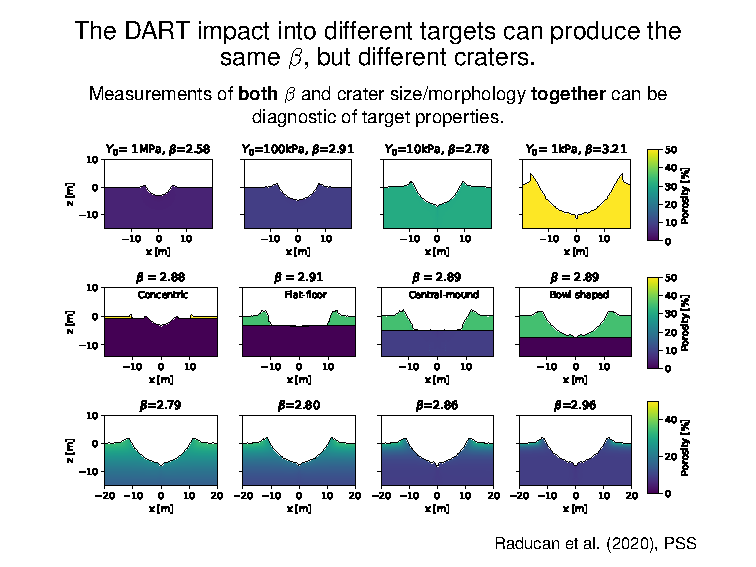
\includegraphics[keepaspectratio,
	width=\paperwidth,
	height=\paperheight]{cratering_raducan.pdf}};
\end{tikzpicture}
\end{frame}

\begin{frame}{Impact angle}
	Not seen in 2d grid codes Raducan
\end{frame}
\begin{frame}{Conclusion}
\end{frame}
\end{document}